% This Source Code Form is subject to the terms of the Mozilla Public
% License, v. 2.0. If a copy of the MPL was not distributed with this
% file, You can obtain one at https://mozilla.org/MPL/2.0/.

\documentclass[a4paper,12pt]{article}
\usepackage[T2A]{fontenc}
\usepackage[utf8]{inputenc}
\usepackage[russian]{babel}
\usepackage{amsmath, amssymb}
\usepackage{geometry}
\geometry{margin=2cm}
\usepackage{array}
\usepackage{booktabs}
\usepackage{caption}
\captionsetup{labelsep=endash, font=small}
\usepackage{siunitx}
\sisetup{output-decimal-marker={.}, round-mode=places, round-precision=5}
\usepackage{graphicx} % основной пакет для картинок
\usepackage{float}


\begin{document}
	
	\quad \textbf{Опыт №1. Влияние концентрации химических веществ на скорость гомогенной химической реакции}
	
	\quad Целью опыта является доказательство справедливости закона действующих масс для реакции, протекающей в водном растворе:
	
	\[
	\mathrm{Na_2S_2O_3 + H_2SO_4 \rightarrow S \downarrow + SO_2 \uparrow + Na_2SO_4 + H_2O}
	\]
	
	\noindent
	\quad В основе экспериментального измерения скорости данной реак­ции лежит определение ее скорости по отношению к изменению
	концентрации коллоидного раствора серы, образующейся в резуль­тате реакции. Результаты измерений приведены в таблице.
	
	
	\begin{table}[h!]
		\centering
		\caption{Данные для опыта №1 (влияние концентрации на скорость реакции)}
		\begin{tabular}{c|c|c|c|c}
		\toprule
		№ &  $n$, отн. ед. &$\tau$, с & $v=\dfrac{1}{\tau}$, с$^{-1}$ & Константа скорости $k=\dfrac{v}{n}$, усл. \\
		\midrule
		1 & 0.154 & 44.68 & \num{0.02238} & \num{0.14533} \\
		2 & 0.308 & 24.11 & \num{0.04148} & \num{0.13466} \\
		3 & 0.462 & 14.66 & \num{0.06821} & \num{0.14765} \\
		\bottomrule
		\end{tabular}
	\end{table}
	
	Из закона действующих масс и быстроты реакции следует, что в нашем эксперименте должно выполняться соотношение:
	
	\[
	v = k \cdot C_{\text{Na}_2\text{S}_2\text{O}_3}^0
	\]
	
	где $v$ – скорость реакции. В нашей серии экспериментов мы наблюдали появление осадка, который становится видимым при определённой концентрации раствора, поэтому:
	
	\[
	v = \frac{\Delta C_s}{\Delta \tau} \sim \frac{1}{\Delta \tau}
	\]
	
	Отсюда следует, что:
	
	\[
	\frac{1}{\Delta \tau} = k \cdot C_{\text{Na}_2\text{S}_2\text{O}_3}^0
	\]
	
	% В теле документа:
	\begin{figure}[H] % H - точное позиционирование, можно использовать [htbp]
		\centering % выравнивание по центру
		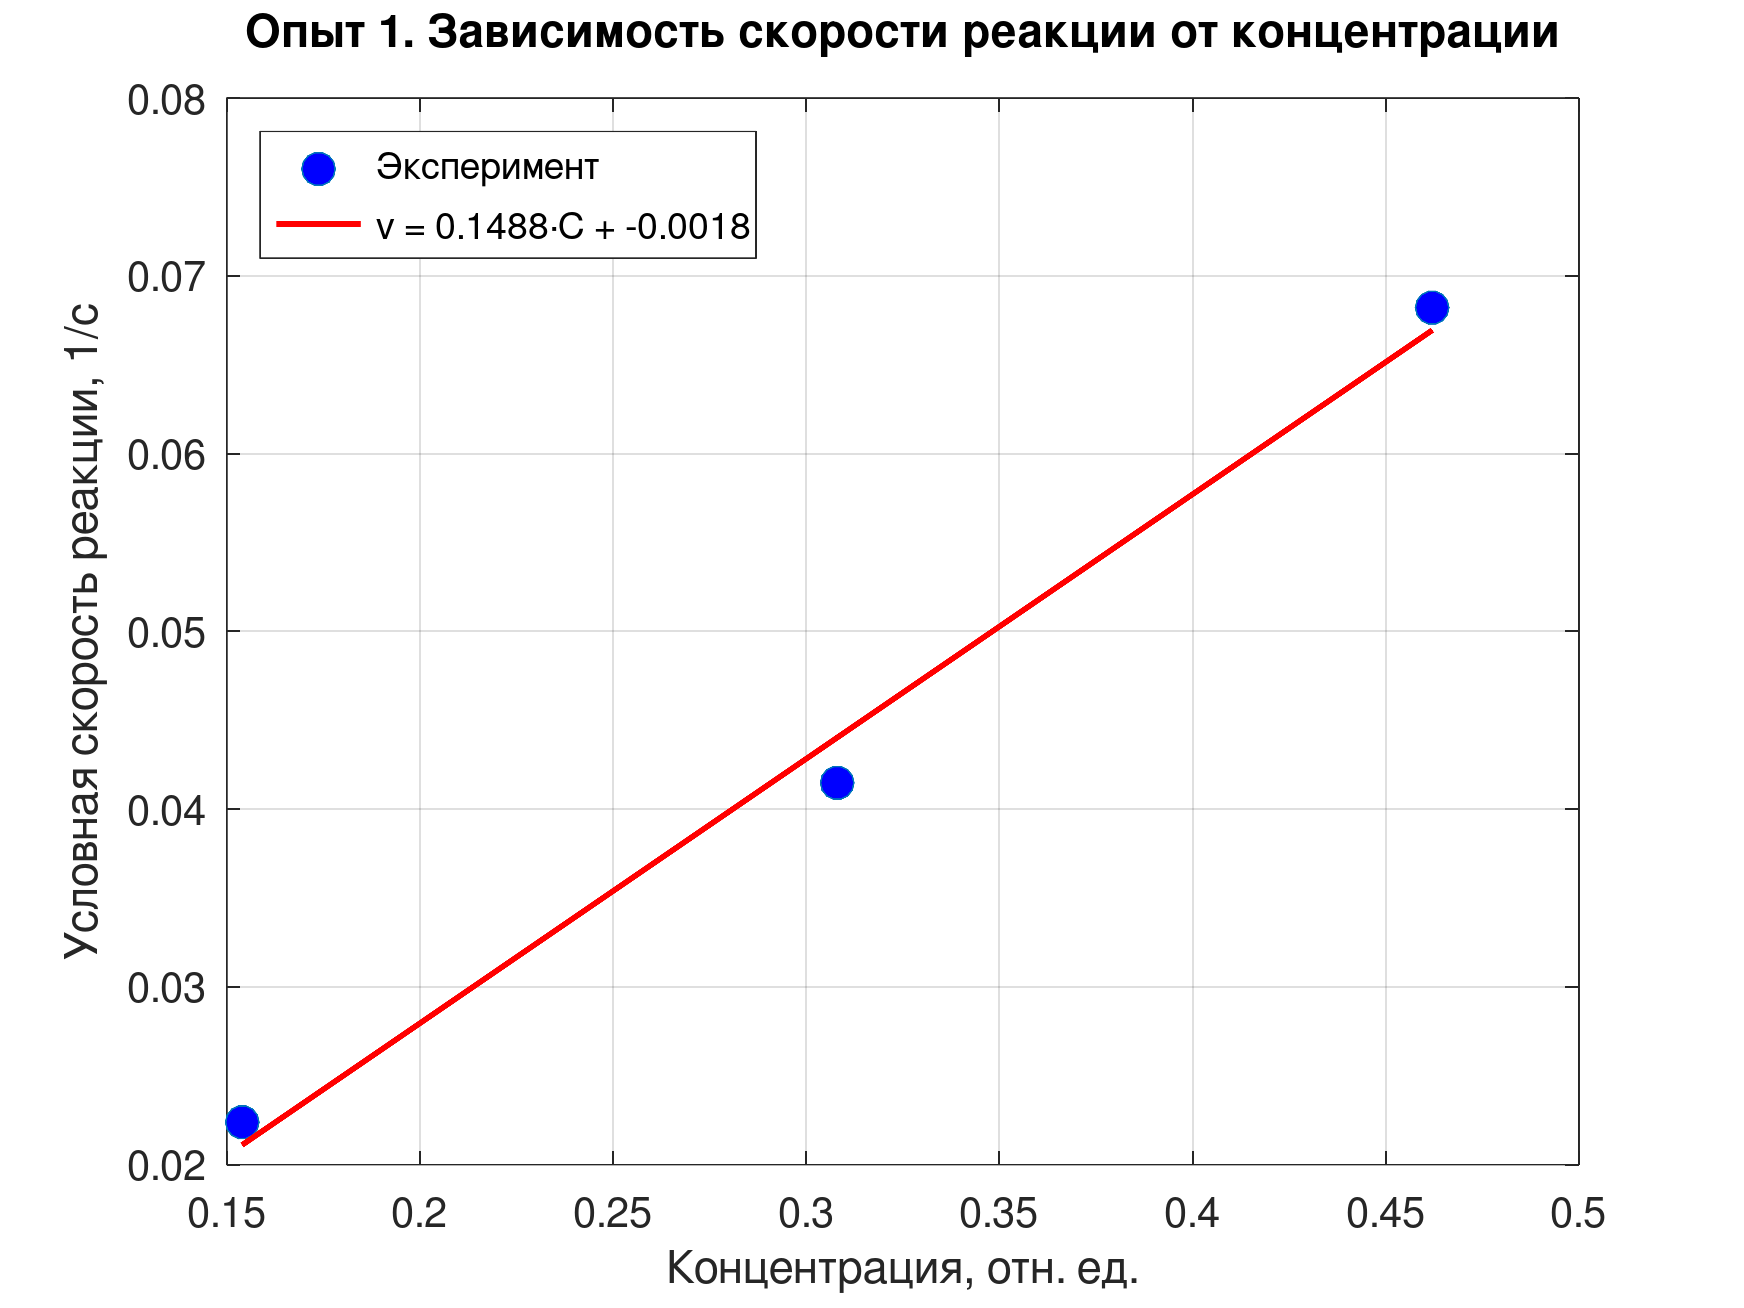
\includegraphics[width=0.6\textwidth]{../../matlab/experiment1_concentration.png} % путь к файлу
		\caption{Апроксимирующая прямая для первого эксперимента} % подпись
		\label{fig:my_image} % метка для ссылок
	\end{figure}
	
	\quad Таким образом подтверждается линейная зависимость между скоростью прохождения реакции от концентрации. Среднее значение константы скорости:
	
	\[
	\langle k \rangle = \frac{\displaystyle\sum\limits_{i=1}^3 k_i}{3} = \frac{0.14533 +  0.13466 + 0.14765}{3} = 0.142546667
	\]
	
	\vspace{1em}
	
	\quad \textbf{Опыт №2. Влияние температуры на скорость гомогенной химической реакции}
	
	Для выяснения влияния температуры на скорость реакции были подготовлены 4 пробирки с одинаковым раствором тиосульфата натрия (4 капли раствора соли на 8 капель воды) и одна пробирка с серной кислотой.
	
	Был подготовлен термостат, состоящий из стакана с водой, закрытого крышкой с тремя отверстиями. В одно отверстие помещён ртутный термометр, во второе -- пробирка с серной кислотой и пипетка для неё, а в третье последовательно помещались пробирки с растворами соли.
	
	Первый опыт был выполнен при комнатной температуре. Затем происходила смена пробирки с раствором соли, нагревание термостата спиртовкой на 10 градусов и повторение эксперимента. Всего измерения были проделаны 3 раза. Эксперимент состоял в добавлении 1 капли серной кислоты в раствор тиосульфата натрия и фиксации времени до выпадения осадка.
	
	\begin{table}[h!]
		\centering
		\caption{Данные для опыта №2 (влияние температуры на скорость реакции)}
		\begin{tabular}{c|c|c|c|c}
			\toprule
			\textbf{Температура, °C} & \textbf{Т K} & \textbf{$\Delta\tau$ с} & \textbf{ $\upsilon$, 1/с} & \textbf{Энергия активации, кДж/моль} \\ \hline
			26 & 299 & 20.00 & 0.050 & 53.1 \\ 
			36 & 309 & 13.00 & 0.0769 & 53.1 \\ 
			46 & 319 & 5.55 & 0.180 & 53.1 \\ 
			\bottomrule
		\end{tabular}
	\end{table}
	
	Рассмотрим влияние температуры на скорость химической реакции. В соответствии с законом действующих масс и уравнением Аррениуса:
	
	\[
	\frac{v(T_2)}{v(T_1)} = \frac{k(T_2)}{k(T_1)} = \frac{A(T_2)e^{-\frac{E_a}{RT_2}}}{A(T_1)e^{-\frac{E_a}{RT_1}}} = \frac{A(T_2)}{A(T_1)} \cdot e^{-\frac{E_a}{R} \left( \frac{1}{T_2} - \frac{1}{T_1} \right)}
	\]
	
	Учитывая, что
	\[
	\frac{v(T_2)}{v(T_1)} = \frac{1/\Delta t_2}{1/\Delta t_1} = \frac{\Delta t_1}{\Delta t_2}
	\]
	равило Вант-Гоффа:
	\[
	\frac{v(T_2)}{v(T_1)} = \gamma^{\frac{T_2 - T_1}{10}}
	\]
	получаем:
	\[
	\gamma = \left( \frac{\Delta t_1}{\Delta t_2} \right)^{\frac{10}{T_2 - T_1}} \tag{1}
	\]
	
	С другой стороны, учитывая температурную зависимость предэкспоненциального множителя в теории активированного комплекса:
	\[
	A(T) = \frac{RTe^{\frac{\Delta S^0}{R}}}{N_A h}
	\]
	где $N_A$ -- постоянная Авогадро, $R$ -- универсальная газовая постоянная, $h$ -- постоянная Планка, $\Delta S^0$ -- стандартное изменение энтропии при образовании активированного комплекса.
	
	Тогда:
	\[
	\gamma = \left( \frac{T_2}{T_1} \right)^{\frac{10}{T_2 - T_1}} e^{\frac{10E_a}{RT_1T_2}}
	\]
	
	Приравнивая выражения (1) и (2), получаем:
	\[
	\left( \frac{\Delta t_1}{\Delta t_2} \right)^{\frac{10}{T_2 - T_1}} = \left( \frac{T_2}{T_1} \right)^{\frac{10}{T_2 - T_1}} e^{\frac{10E_a}{RT_1T_2}}
	\]
	
	После преобразований:
	\[
	\left( \frac{\Delta t_1 T_1}{\Delta t_2 T_2} \right)^{\frac{10}{T_2 - T_1}} = e^{\frac{10E_a}{RT_1T_2}}
	\]
	
	Логарифмируя обе части уравнения:
	\[
	\frac{10}{T_2 - T_1} \ln \frac{\Delta t_1 T_1}{\Delta t_2 T_2} = \frac{10 E_a}{RT_1 T_2}
	\]
	
	Откуда энергия активации:
	\[
	E_a = \frac{R T_1 T_2}{T_2 - T_1} \ln \frac{T_1 \Delta t_1}{T_2 \Delta t_2} \tag{2}
	\]
	
		% В теле документа:
	\begin{figure}[H] % H - точное позиционирование, можно использовать [htbp]
		\centering % выравнивание по центру
		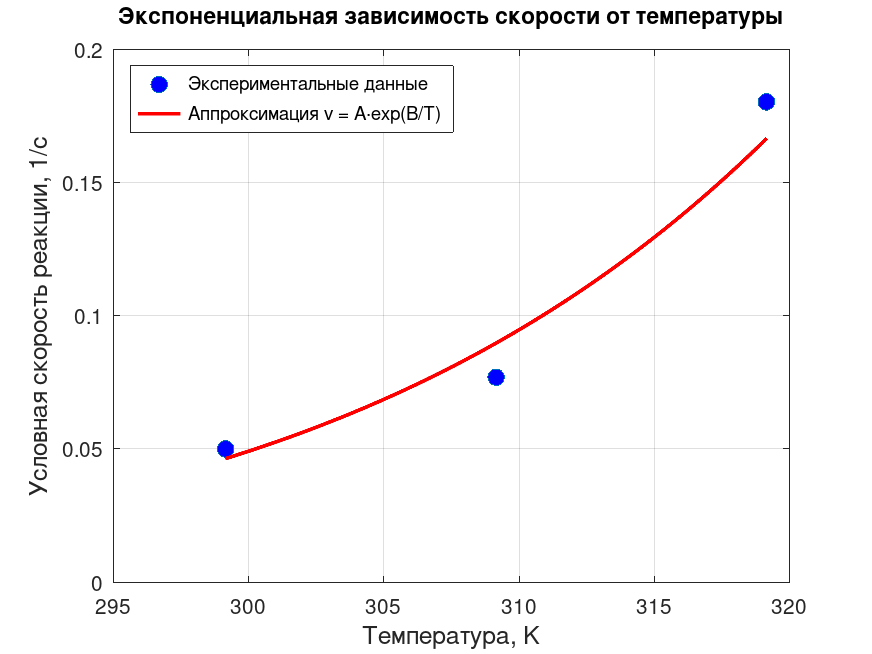
\includegraphics[width=0.6\textwidth]{../../matlab/exp_fit.png} % путь к файлу
		\caption{Апроксимирующая кривая для второго эксперимента} % подпись
	\end{figure}
	
	
	\vspace{1em}
	
	\quad \textbf{Выводы}
	
	В ходе лабораторной работы изучено влияние концентрации реагентов и температуры на скорость гомогенной химической реакции. Экспериментально подтверждено, что:
	
	\begin{itemize}
		\item скорость реакции прямо пропорциональна концентрации реагирующего вещества;
		\item скорость реакции возрастает с увеличением температуры, что согласуется с правилом Вант-Гоффа;
		\item рассчитанные значения температурного коэффициента и энергии активации находятся в допустимом теоретическом диапазоне.
	\end{itemize}
		
	
	
\end{document}
